\section{Experimental Results}

\textcolor{red}{(TODO: performance results are not included in section 6. we
should add some numbers such as runtime, throughput, cdf of latency, and SW
overhead)}

We have implemented \textsf{PCStream} on the Linux kernel 4.5 that runs on
Intel's i7-2600 CPUs with 8 cores and with 16~GB DRAM.  Samsung's PM963 480~GB
SSD with a multi-stream feature is used.  PM963 supports up to 9 streams; 8
user-configurable streams and one default stream. Write requests that do not
specify their stream IDs are assigned the default stream.  To support the
internal stream, we have modified the SSD firmware.  For detailed performance
analysis, an \texttt{nvme-cli} tool is modified to retrieve the information of
\textsf{PCStream}-enabled device internals, such as the WAF or
\textcolor{red}{the valid time of data in every blocks}.

%and its firmware has been modified to
%support the internal stream.

For an objective evaluation, we compared \textsf{\small PCStream} with three
existing schemes: \textsf{\small Baseline}, \textsf{\small
ManualStream}~\cite{MultiStream}, and \textsf{\small
AutoStream}~\cite{AutoStream}.  \textsf{\small Baseline} stands for a legacy
SSD that does not support multiple streams. \textsf{\small ManualStream}
represents multi-streamed SSDs with manual stream allocation.  \textsf{\small
AutoStream} is one that employs an LBA-based data separation technique which is
implemented at the device driver layer. 

We have carried out experiments with various benchmark programs, including
RocksDB~\cite{}, Cassandra~\cite{}, SQLite~\cite{}, and GCC~\cite{}, each of
which generates distinct write patterns.  RocksDB and Cassandra have
append-only write patterns; SQLite has in-place update write patterns; GCC has
a write-once pattern.  We also run the combinations of multiple programs
simultaneously for assessments under more realistic environments.  Yahoo! Cloud
Serving Benchmark (YCSB)~\cite{YCSB} with 120,000,000 keys runs on top of
RocksDB and Cassandra.  Both RocksDB and Cassandra are based on the LSM-tree
algorithm, so they have three major I/O activities (e.g.,
\textcolor{red}{logging, flush, and compaction}) as analyzed in Section 3.
%However, we identified about 5 PCs during runtime and we consider the extra
%PCs as management use.
TPC-C~\cite{TPCC} runs on SQLite with 20 warehouses.  Similarly, SQLite has two
major I/O activities (e.g., \textcolor{red}{logging and YYY}). 
%2 kinds of data types in theory but we identified 4 PCs.
GCC compiles kernel source code 30 times. For the each run, 1/3 of source files
that are randomly chosen are modified and involved in the compilation.  GCC
creates many temporary files (e.g., \textcolor{red}{XXX}) as well as long-lived
files (e.g., \textcolor{red}{YYY}), thereby having more than 20 PCs.  To
generate mixed workloads, we run RocksDB and GCC scenarios together (denoted by
Mixed 1), and run SQLite and GCC scenarios at the same time (denoted by Mixed
2).
%Since GCC writes many kinds of temporary files as well as long-lived files,
%GCC has more than 20 PCs which makes clustering process effective for the GCC
%and mixed workloads.
To emulate an aged SSD, 90\% of the total SSD capacity was initially filled up
with user files before benchmarks run.


\subsection{WAF Comparison}

\begin{figure}[t]
	\centering
	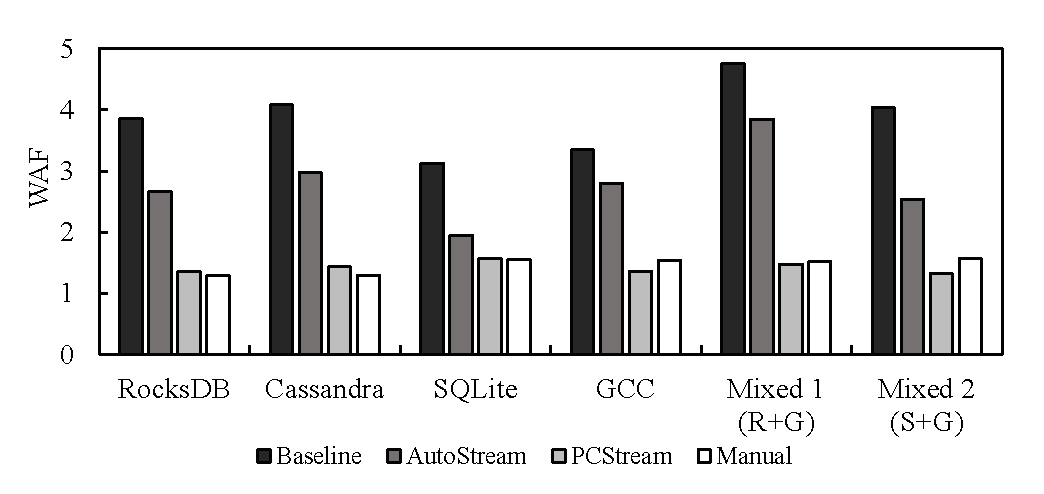
\includegraphics[width=0.9\linewidth]{figure/waf}
	\caption{The WAF comparison for various workloads.}
	\label{fig:waf}
	%\vspace{-36pt}
\end{figure}

We compared WAF of the existing techniques with \textsf{\small PCStream} for
various workloads and the result is shown in Fig.~\ref{fig:waf}.
\textsf{\small PCStream} was quite effective in reducing WAF, thus achieving an
equivalent level of the WAF reduction as in \textsf{\small Manual}.  For
example, \textsf{\small PCStream}  reduced WAF by 63\% over \textsf{\small
Baseline} on average.  \textsf{\small PCStream} also outperformed
\textsf{\small AutoStream} by reducing WAF by 49\% on average.  The result
shows that separating short-lived data (e.g., log or temp files) from
long-lived one (e.g., compaction or result files) using PC was quite effective
in reducing WAF.  Moreover, \textsf{\small PCStream} even showed similar WAF to
\textsf{\small Manual}, reducing it by up to 69\% over \textsf{\small
AutoStream} for \texttt{Mixed 1} case.

AutoStream was not able to achieve high WAF reduction because of 
the lack of relationship between hotness and address in the general I/O workloads.
As a result, AutoStream showed WAF larger than 2 for all the cases except SQLite.
Only SQLite has in-place update pattern for log files, but the larger amount of data are
written for database files whose lifetimes are determined by the client
which makes hard to predict their lifetime by the address.
In PCStream, however, long-lived data in database files are moved to internal streams
during GC so that we can further reduce WAF.

For GCC and mixed workloads, PCStream achieved even better than Manual
since the Manual scheme has static stream allocation.
In Manual, once data types is mapped to the stream, the mapping is not changed 
during runtime.
For complex workloads which have large number of PCs such as mixed cases,
it is difficult to expect data lifetimes in detail based on the data types.
If the lifetime pattern is changed during runtime or the programmer choose
second best stream mapping,
Manual scheme lose the potential benefit in reducing WAf.
However, the reclustering enables PCStream to adapt changing workload or find
better stream mapping.
The detailed analysis will be shown in the following subsections.

\begin{comment}
For example, both \textsf{\small PCStream} and \textsf{\small Manual} reduced WAF by 38\% over \textsf{\small Baseline} for the \texttt{UR} case. 
Compared with \textsf{\small AutoStream}, \textsf{\small PCStream} was more effective, reducing WAF more by 35\% on average.  
\textsf{\small PCStream} outperformed \textsf{\small AutoStream} by reducing WAF by 35\% on average.
Fig. 6 also indicates that the two-phase stream assignment technique is effective.  
\textsf{\small PCStream} outperformed \textsf{\small PCStream$^{*}$} by 12\% on average in the WAF reduction.
As shown in Fig. 6, \textsf{\small PCStream$^*$} reduced WAF by up to 30\% over \textsf{\small AutoStream}.  
\end{comment}

\subsection{Per-stream Lifetime Distribution Analysis}

\begin{figure}[t]
	\centering
	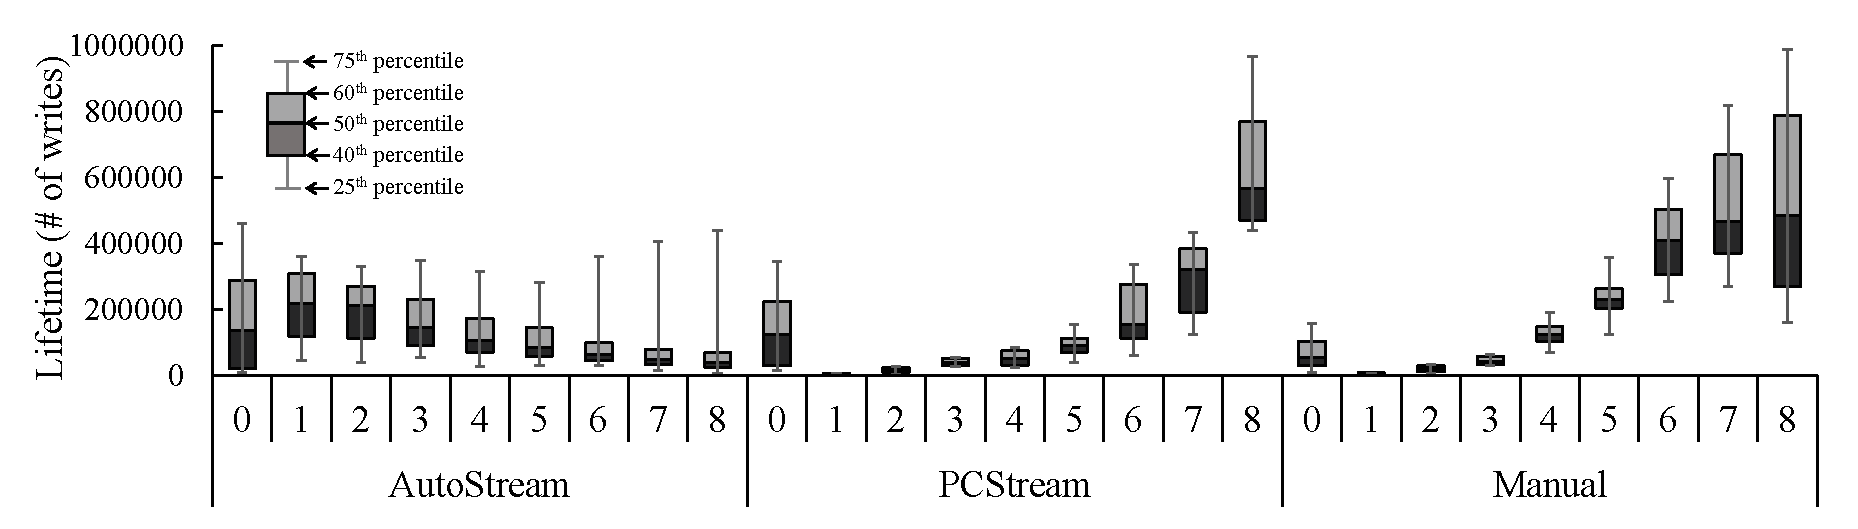
\includegraphics[width=1\linewidth]{figure/distribution}
	\caption{A Comparison of lifetime distributions of the smaller variance streams.}
	\label{fig:distribution}
	%\vspace{-36pt}
\end{figure}

In order to better understand how \textsf{\small PCStream} achieved a high reduction in WAF, 
we measured per-stream lifetime distributions under each 
technique for the \texttt{Mixed 1} scenario.
Fig.~\ref{fig:distribution} shows a box plot of data lifetimes from the 
25th percentile to the 75th percentile.
As shown in Fig.~\ref{fig:distribution}, 
streams in both \textsf{\small PCStream} and Manual are divided into two groups, 
$G1$ = $\{$1, 2, 3, 4, 5$\}$ and $G2$ = $\{$6, 7, 8$\}$, 
where $G1$ includes streams with short lifetimes and small variances 
(i.e., streams 1, 2, 3, 4, and 5) 
and $G2$ includes streams with large lifetimes and large variances (i.e., streams 6, 7, and 8).  
In PCStream, every streams especially streams in G2 showed smaller variance than 
Manual.
This is because long-lived data in those streams are moved to internal streams, thus 
reducing the lifetime variance.
Since the GC copy cost is affected by how data in $G1$ and $G2$ are mixed into the same block, 
\textsf{\small PCStream} can significantly reduce the GC overhead 
by avoiding such data mixtures in the same block by separating $G1$ and $G2$ into different streams. 

On the other hand, AutoStream was not able to achieve small variance of data lifetimes in a stream.
AutoStream allocates data in a address range to stream 1 at first.
The data will be allocated to stream 2 when the frequency of the range hits the 
pre-defined threshold which means the address range holds hotter data.
However, since there is no strong relation between hotness of data and the address in RocksDB
or GCC workload, 
long-lived data can be placed to the hot address range which results 
very high lifetime variances for all the streams.
Since a block with very small number of valid pages will be easily involved to GC,
long-lived data in stream 8 is the worst case scenario 
for preventing valid page copies during GC.

\subsection{Analysis of the Internal Stream Impact}

In order to understand the impact of the two-phase assignment, we compared each
technique with and without the internal stream.  The internal stream works
independently of a stream assignment method running at the host level, so it
can easily be combined with any host-level techniques.  Fig.~\ref{fig:internal}
shows a comparison of WAF values of Baseline, AutoStream, and PCStream under
the five workloads.  At a glance, we notice that all the techniques benefited
from using the internal stream.  However, its impact was not so high to offset
WAF costs caused by the improper stream assignment by the first-phase.  For
example, in Baseline, all the data from the host are first written to the same
default stream, regardless of their hotness.  Then, during SSD GC, cold data
that are left valid in the default stream are moved to the internal stream.
This helps us prevent cold data from being mixed up with future incoming data,
separating hot and cold data in two different segments. However, since the host
keeps writing the mixture of hot/cold data to the default stream, it is
impossible to avoid extra copy costs involved in the default stream.
AutoStream worked better than Baseline by assigning hot and cold data to
different streams, but owing to the inaccuracy of LBA-based hot-cold detection,
it performed worse than PCStream.

\begin{figure}[t]
	\centering
	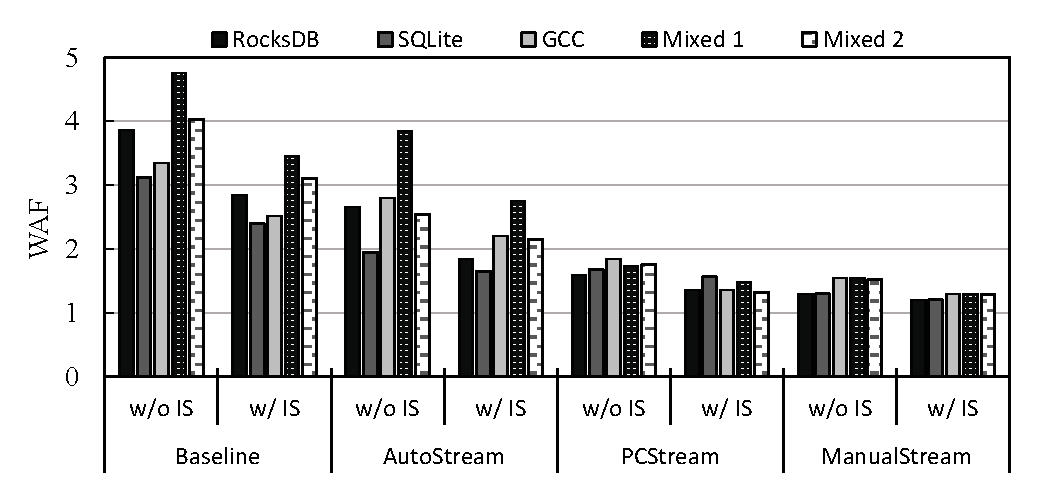
\includegraphics[width=0.9\linewidth]{figure/internal}
	\caption{An WAF comparison with and without using internal streams.
		\textcolor{red}{(TODO: How about adding
		the improvement ratio (\%) instead of showing absolute WAF numbers?)} 
	}
	\label{fig:internal}
	%\vspace{-36pt}
\end{figure}


\subsection{Analysis of the PC-stream table Impact}

\begin{figure}[t]
	\centering
	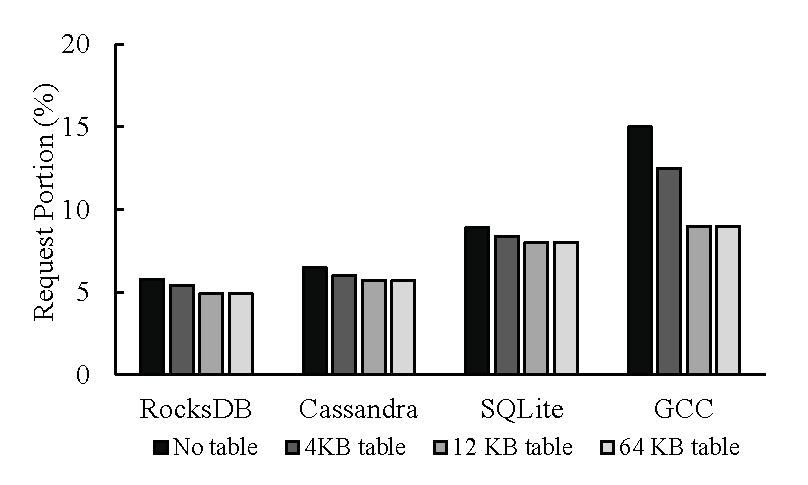
\includegraphics[width=0.7\linewidth]{figure/pctable}
	\caption{Request portion comparison of stream 0 with PC-stream table.
		\textcolor{red}{(TODO: How about adding the size of PC-stream table? It was mentioned in
		the text of the paper.)} }
	\label{fig:pctable}
	%\vspace{-36pt}
\end{figure}

As explained in Section 5, PCStream can benefit from the uniqueness of PCs
by using the PC-stream table.
PCs of frequently launched and terminated process can be directly allocated without
waiting for sufficient lifetime values are collected.
Fig.~\ref{fig:pctable} shows the request portion of stream 0, where 
awaiting requests are allocated.
As shown in Fig.~\ref{fig:pctable}, DB applications run 
continuously so the benefit of using PC-stream table was very small. 
However, since GCC is executed repeatedly, 6 percent of requests are directly
allocated to the desinated streams based on the lifetime information from the 
previous execution. 
Due to the direct allocation with PC-stream table, PCStream can 
reduce WAF from 1.96 to 1.54 for GCC workload.


